\section{Method}
\label{sec:method}


\subsection{Problem Formulation}

We first define the setting and notations for vision-language-action (VLA) reasoning tasks. At each timestep $t$, the model receives a visual observation $o_t$ and a textual instruction $l$, with the goal of predicting an action $a_t$, which can be a textual command or a 7-DOF control vector $\left[ \Delta_x, \Delta_\theta, \Delta_\text{Grip} \right]$ depending on the embodiment.
To tackle this problem, we propose \textit{\ours{}}, a unified framework that aims to leverage an MLLM $\mathcal{F}_\theta$ to reason the high-level plans while connecting with an action model $\pi_\phi$ to infer executable actions. The MLLM $\mathcal{F}_\theta$ produces a visual plan latent $c_t$ based on $(o_t, l)$, capturing the high-level intent and planning context (Sec.~\ref{ssec:ER}). This reasoned plan $c_t$ then guides the downstream action module $\pi_\phi$ to sequentially predict $N$ executable actions $[a_t]_{t}^{t+N}$ tailored to the target environment (Sec.~\ref{ssec:action}). By connecting abstract planning with low-level control, our \ours{} enables long-horizon reasoning and improves action adaptation in dynamic embodied tasks.



\subsection{Reinforced Visual Latent Planning for Embodied Reasoning}
\label{ssec:ER}

\begin{figure}[t!]
    \centering
    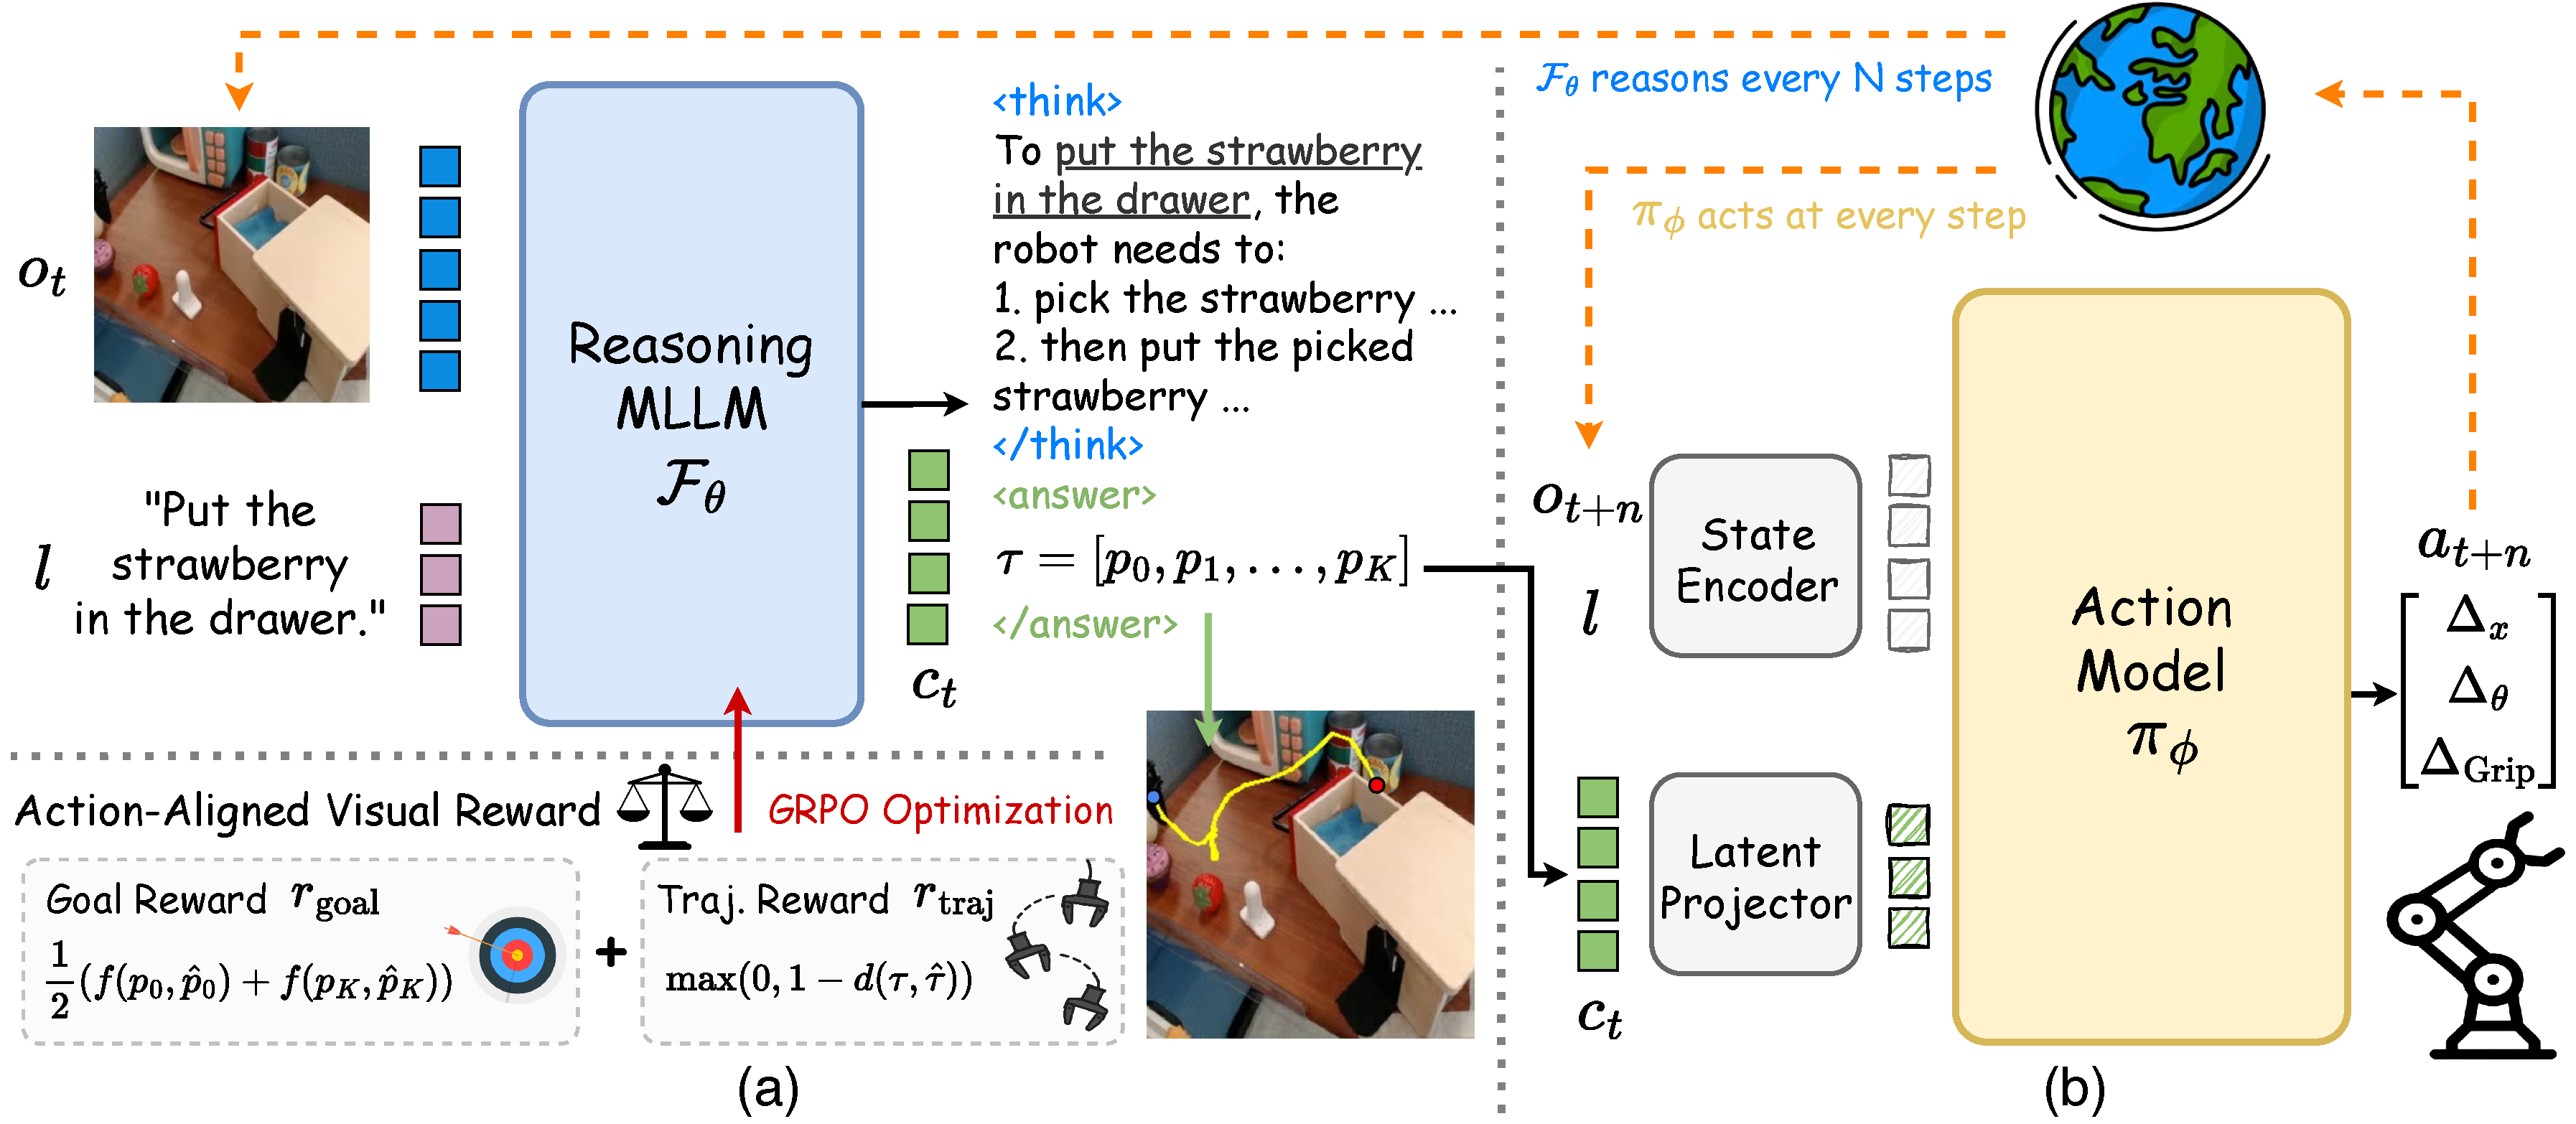
\includegraphics[width=1.0\linewidth]{figures/images/overview.pdf}
    \caption{\textbf{Overview of our \ours{}.} (a) Given observation $o_t$ and instruction $l$, \ours{} advances \emph{action-aligned} rewards derived from visual trajectory $\tau$ to incentivize embodied reasoning capability of Reasoning MLLM $\mathcal{F}_\theta$. (b) Conditioned on the visual plan latent $c_t$, the DiT-based Action Model $\pi_\phi$ learns to predict executable action while keeping $\mathcal{F}_\theta$ frozen. Note that, during inference, $\pi_\phi$ and $\mathcal{F}_\theta$ could operate asynchronously to enable slow thinking and fast control for VLA reasoning tasks.}
    \label{fig:overview}
\end{figure}



To enable embodied reasoning that generalizes across diverse environments, we aim to incentivize the reasoning capability of multimodal LLMs via reinforcement learning~\cite{shao2024deepseekmath,guo2025deepseek}. A straightforward way is to have the MLLM reason before generating low-level actions, while using the resulting task success rate in target environments (e.g., LIBERO~\cite{liu2023libero}) as the reward signal. However, this approach is restricted to specific simulators without proper guidance from visual scenes.

\paragraph{Reward Shaping from Action-Aligned Visual Feedback}
To tackle this challenge, we design a novel action-aligned visual feedback that captures long-horizon goals and encourages visual grounding during planning. Specifically, inspired by recent works~\cite{yang2025magma,zheng2024tracevla}, we are capable of representing high-level plans as spatial-temporal trajectories that capture the gripper end-effector over the visual scene, which serve as a visual-action guidance to steer the embodied reasoning.


As depicted in Fig.~\ref{fig:overview}(a), given an observation $o_t$ at timestep $t$ and a task instruction $l$, the MLLM $\mathcal{F}_\theta$ autoregressively generates a sequence of latent embeddings for reasoning $v_t \in \mathbb{R}^{|v_t| \times d}$ and visual plan $c_t \in \mathbb{R}^{|c_t| \times d}$, where the former is decoded to reasoning steps while the latter would be inferred into a text string of 2D points $\tau = \left[p_k\right]_{k=1}^K$, with $p_k \in [0, 1]^2$, and $p_1$ and $p_K$ denoting the \emph{start} and \emph{end} positions of the gripper.
As a result, to encourage the model to anticipate visual goal completetion, we introduce the \emph{goal reward} for comparing  predicted start and end positions with corresponding points from trajectory obtained by off-the-shelf detector~\cite{niu2024llarva} $\hat{\tau} = \left[\hat{p}_k\right]_{k=1}^K$ as follows,
\begin{equation}
    r_{\text{goal}} = \frac{1}{2} \left( f\left( p_1, \hat{p}_1 \right) + f\left( p_K, \hat{p}_K \right) \right), \quad \text{where } f(p, p^\prime) = \max\left( 0, 1-\| p - p^\prime \|_2^2 \right).
\end{equation}


To further enforce the MLLM predicted trajectory to properly correspond to physically plausible gripper motion, the \emph{trajectory reward} is proposed to regularize the predicted $\tau$ to match the distribution of demonstrated trajectory $\hat{\tau}$. Thus, the trajectory reward $r_{\text{traj}}$ can be computed as follows,
\begin{equation}
    r_{\text{traj}} = \max\left( 0, 1 - d(\tau, \hat{\tau}) \right).
\end{equation}
Here, $d(\tau, \hat{\tau})$ denotes a metric measuring the distance between two trajectories, i.e., dynamic time warping (DTW) distance~\cite{senin2008dynamic} in this work.

The overall reward is thus defined as the combination of our proposed action-aligned visual feedback and the format correctness score $r_\text{format}$ following existing reasoning works~\cite {guo2025deepseek}:
\begin{equation}\label{eq:reward_total}
    r = 0.9 r_\text{visual} + 0.1 r_\text{format}, \text{where }r_\text{visual} = \omega_\text{goal}r_\text{goal} + \omega_\text{traj}r_\text{traj}.
\end{equation}
Here, $\omega_\text{goal} = \omega_\text{traj} = 0.5$ are the weighting coefficients for the goal and trajectory rewards.

\paragraph{Reinforced Fine-Tuning for Eliciting Visual Latent Planning}

To incentivize the embodied reasoning from the MLLM $\mathcal{F}_\theta$, we perform reinforced fin-tuning using Group Relative Policy Optimization (GRPO)~\cite{shao2024deepseekmath}.
Specifically, given an input $(o_t, l)$, GRPO first samples a group of $M$ distinct responses $\{ z_1, z_2, \ldots, z_M \}$ from the original MLLM $\mathcal{F}_{\theta_\text{old}}$. Each response is evaluated using the reward function defined in Eq.~\ref{eq:reward_total} and resulting in a set of reward signals $\{ r_1, r_2, ..., r_M \}$. Thus, we optimize $\mathcal{F}_{\theta}$ by maximizing the following objective:
\begin{equation}
    \mathcal{J}_\text{GRPO}(\theta) = \frac{1}{M} \sum_{i=1}^{M}(\frac{\mathcal{F}_{\theta}(z_i|o_t,l)}{\mathcal{F}_{\theta_\text{old}}(z_i|o_t,l)}A_i - \beta D_{KL}(\mathcal{F}_{\theta}(z_i|o_t,l)\parallel \mathcal{F}_{\theta_\text{old}}(z_i|o_t,l))),
\end{equation}
\begin{equation*}
     \\ \text{where} \quad A_i=\frac{r_i - \text{mean}(\{ r_1, \ldots, r_M \})}{\text{std}(\{ r_1, \ldots, r_M \})}.
\end{equation*}
Here, $A_i$ quantifies the relative quality of $i$-th response compared to other candidates in the sampled group. $D_{KL}(\cdot\parallel\cdot)$ is the KL divergence introduced with a weighting factor $\beta$ to regularize the model, preventing excessive deviation from the original model $\mathcal{F}_{\theta_\text{old}}$.

To further obtain general embodied knowledge, our \ours{} is flexible to encapsulate the publicly available question-answering data to enhance capabilities such as robotic VQA~\cite{sermanet2024robovqa} or failure detection~\cite{liu2023reflect} by formatting them into the QA-style accuracy reward. Once the reinforced fine-tuning is complete, we are able to produce long CoT steps, while abstracting the textual reasoning into a compact visual plan latent $c_t$, capturing long-horizon spatial-temporal planning intent.  


\subsection{Reasoning-Enhanced Action Adaptation}
\label{ssec:action}

With the high-level embodied intent reasoned by the MLLM, our goal is to connect the inferred visual latent planning $c_t$ with the action model $\pi_\phi$ of the target environment in a think-before-acting manner, grounding embodied reasoning into the physical world with executable actions.
Specifically, we build upon a Transformer-based action model $\pi_\phi$ (e.g., Diffusion Policy~\cite{chi2023diffusion}), which predicts actions based on the current state composed of visual observations and language instructions. While $\pi_\phi$ can operate in the target environment using perception alone, we enhance its capability by conditioning it on the latent plan $c_t$, which encodes high-level embodied intent and planning context.

As depicted in Fig.~\ref{fig:overview}(b), we incorporate $c_t$ using a latent projector to connect it to the input space of the action model, enabling the reasoning guidance to be effectively leveraged, which enhances its low-level action execution in the target environment. Thus, we solely update the state encoder, latent projector, and action model by imitation learning with annotated action demonstrations: 
\begin{equation} \mathcal{L}_{\text{IL}}(\phi) = \mathbb{E}_{(o_i, l, a_i)} \left[ \ell\left(\pi_\phi(c_{t}, o_i, l), a_i \right) \right]. \end{equation} 

We note that, reasoning and action execution could be operated in an \textit{asynchronous} manner, which means each latent plan $c_t$ corresponds to $N$ interactions with the environment (i.e., $i\in[t, t+N]$). This asynchronous design highlights a key advantage of our dual-system architecture, allowing the reasoning MLLM to perform slow thinking while the action model executes fast control.



\subsection{Learning Strategy and Inference}

Following~\cite{feng2025video}, we adopt a multi-stage training strategy for our \ours{}. Before RL, we initialize the two modules independently. The MLLM $\mathcal{F}_\theta$ is cold-started using supervised data (Sec.~\ref{ssec:exp_setup}) to learn to interpret visual trajectories and produce reasoning and answers in the correct output format. On the other hand, the action model $\pi_\phi$ is pre-trained on the Open X-Embodiment (OXE) dataset~\cite{o2024open}, providing a strong foundation for low-level action execution.
After SFT cold-start, our MLLM $\mathcal{F}_\theta$ is tuned with action-aligned rewards guiding the generation of effective latent plans. During reasoning-enhanced action adaptation, we freeze $\mathcal{F}_\theta$ while updating the action model $\pi_\phi$ with state encoder and latent projector on the target environment by conditioning on the latent visual plan $c_t$.

At inference time, given a visual observation $o_t$ and instruction $l$, \ours{} produces a visual plan latent $c_t = \mathcal{F}_\theta(o_t, l)$, which conditions the action module $\pi_\phi$ to predict a sequence of executable actions tailored to the current environment.